% -----------------------------------------------------------------------
% -----------------------------------------------------------------------
% -----------------------------------------------------------------------
% Einleitung
% -----------------------------------------------------------------------
% -----------------------------------------------------------------------
% -----------------------------------------------------------------------
\chapter{Introduction: An Open-Domain Comparative Argumentative Machine (CAM)}
This thesis discusses the topic of \emph{comparative argument mining}. Comparative argument mining is a subfield of \emph{argument mining}, a recent research topic in natural language processing.

The goal is to develop a system which is able to decide if a given sentence compares two known objects and, if it does, which object wins the comparison. For instance, given the sentence \emph{\enquote{In my mind, Python is better than Java!}}, the system should answer that the sentence is comparative and that Python won the comparison.

Such a system can be useful in several ways. First, it enables machines to understand the statements of such sentences. Second, this knowledge can be used in (commercial) applications, like opinion mining or online comparison portals. As presented in Section \ref{sec:domainspec}, these portals usually rely on information from databases. The system presented in this thesis could be used to generate new knowledge automatically from forum posts, comments, tweets and the like. Furthermore, this new knowledge would include the thoughts and opinions of their authors. This stands in contrast to the pure factual information from databases. For instance, the system could find out that many people complain about the telephone support of insurance company X, while they praise the support of company Y - an information rarely found in databases.\newline

The thesis is structured into three main parts. The first part discusses recent publications in argument mining and explains the needed concepts from natural language processing and machine learning.

Because comparative argument mining is a novel field, no suitable data set for this task currently exists. The second part describes the creation of a data set with data crawled from the web and crowdsourcing methods to label the data. The result is a data set with 7199 sentences, containing comparisons of 271 object pairs. Each sentence is annotated with one of three classes (\texttt{BETTER}, \texttt{WORSE}, \texttt{NONE}) which reflects whether the sentence is comparative and whether the first mentioned object in the sentence won the comparison.

The third part uses this data set to train machine learning models on several feature representations in order to predict the correct class. As the final evaluation, all features are tested on held-out data.

\chapter{Background}
\section{Related Work}
\label{sec:argth}
\label{sec:argmine}
In the following, publications on argument mining are presented. If appropriate, the f1 scores achieved in these publications are presented as well. It must be noted that the f1 scores are not comparable with each other.

A general introduction on the research topic argument mining was given in \cite{Lippi2016Argumentation-M}.
The authors introduced five dimensions to describe argument mining problems: granularity of input, the genre of input, argument model, the granularity of target and goal of analysis.  Furthermore, the typical steps of argument mining systems were described. First, the input is divided into argumentative (e.g. claim and premise) and non-argumentative parts. This step was described as a classification problem. Second, the boundaries of the argumentative units must be identified; this was understood as a segmentation problem. Third, the relations between argumentative units must be identified. For instance, claims and premises might be connected with a \emph{support} or a \emph{attack} relation.


%07 biomed

A system, which is capable of recognising comparative sentences and their components such as the compared entities, the property which is used to compare the entities and the direction of comparison, was presented in \cite{fiszman2007interpreting}. The evaluation showed that the outcome has a high quality (f1 score of 0.81). However, the presented system was specific to the domain of studies on drug therapy. The system used patterns generated from hand-selected sentences, as well as domain knowledge. Therefore, the methods cannot be transferred easily to the problem of this thesis.

%  12 sci
In \cite{park2012identifying}, the authors presented another domain-specific approach on argumentative sentence detection. The problem was formulated as a binary classification task. As in \cite{fiszman2007interpreting}, the features were tailored for medical publications.

The authors conducted a pilot study with 274 comparison sentences extracted from abstracts and 164 comparison sentences from full text articles. The sentences were analysed in order to extract 35 features (six lexical features, 27 syntactic features and two miscellaneous features). For instance, a lexical feature capturing the appearance of \emph{\enquote{versus}} or \emph{\enquote{vs.}} was developed, while a miscellaneous feature checked if the subject of the comparison is in plural. 


% 10 biomed
A recent publication on comparative argument mining is \cite{gupta2017identifying}, were a set of rules for the identification of comparative sentences (and the compared entities) was derived from syntactic parse trees. With these rules, the authors achieved a f1 score of 0.87 for the identification of comparative sentences. The rules were obtained from 50 abstracts of biomedical papers. Such being the case, they are domain dependent.\newline

The challenges occurring while processing texts from social media were described in \cite{Snajder2017Social-Media-Ar}. Besides the noisiness of text, missing argument structures and poorly formulated claims were mentioned. It is expected that the text used in this thesis will have the same shortcomings. Additionally, \cite{Snajder2017Social-Media-Ar} emphasized that analyzing social media texts can delivery reasons behind opinions.

In addition to the challenges mentioned above, \cite{Dusmanu2017Argument-Mining} also pointed to the specialized jargon in user-generated content like hashtags and emoticons. With this in mind, \cite{Dusmanu2017Argument-Mining} classified tweets about the \enquote{\emph{Brexit}} and \enquote{\emph{Grexit}} either as argumentative or as non-argumentative. Beside features used in other publications mentioned in this section, new features covering hashtags and sentiment were added. They achieved a f1 score of 0.78 (using logistic regression) for the classification. It must to be mentioned that the data set is small (1887 tweets) and the domain is rather specific.\newline

Publications dealing with the identification of argument structures are of relevance for this thesis, as they provide valuable insights on the suitability of features and algorithms.

%what works and what does not
The authors of \cite{Aker2017What-works-and-} summarised and compared features used in other publications for identification of argumentative sentences. In addition to the algorithms used in the publications, a convolutional neural network (as described in \cite{Kim2014Convolutional-N}) was tested. Two existing corpora and six different classification algorithms were used. The comparison resulted in the insight that structural features and random forests worked the best.

A two-step procedure to identify components of arguments (such as claim and premise) and their relationships (like \enquote{premise A supports claim B}) is presented in \cite{Stab2014Identifying-Arg}. The identification step is formulated as a multi-class classification. For the identification of argumentative components, a f1 score of 0.72 was reported.

%essence of a claim
How different datasets represent the argumentative unit of a claim was analysed in \cite{Daxenberger2017What-is-the-Ess}. After an analysis of the data sets and their annotation scheme, the authors conducted two experiments.
In the first one, each learner was trained and evaluated (10-fold cross-validation) on each dataset one after another. On average, the macro f1 score for the identification of claims was 0.67 (all results ranging from 0.60 to 0.80). No significant difference between the results of logistic regression and the neural networks was found. In isolation, lexical features, syntactical features and word embeddings were most helpful. Structural features turned out to be the weakest.
The second experiment was conducted in a cross-domain fashion. For each pair of data sets, one was used as the training set and the other one as the test set. The average macro f1 score was 0.54. In this scenario, the best feature combination outperformed all neural models. The authors assumed that there might not be enough training data for the neural models.
As the last point, the authors noted that all claims share at least some lexical clues.


The role of discourse markers in the identification of claims and premises were discussed in \cite{Eckle-Kohler2015On-the-Role-of-}. A discourse marker is a word or a phrase which connects discourse units. For instance, the word \enquote{as} can show a relation between claim and premise: \enquote{As the students get frustrated, their performance generally does not improve}.  A similar function is expected for words like better, worse or because in this thesis. The authors showed that discourse markers are good at discriminating claim and premises. If claim and premise are merged into one class \enquote{argumentative}, this can be used to identify argumentative sentences. The f1 score is not presented, but the accuracy is between 64.53 and 72.79 percent.



\section{Domain-Specific Comparative Systems}
\label{sec:domainspec}

Comparison portals are a possible application for comparative argument mining. Many comparison portals can be found on the internet. It is not unusual to see a television commercial of those comparison portals, which suggests that they are used frequently every day.

Most portals are specific to a few domains and a subset of properties, for example, car insurances and their price. Comparisons are only possible between objects of the domains and predefined properties. Source of the data is usually databases. Humans are involved in gathering, entering and processing the data.

Comparison portals only compare and deliver facts. Because of that, they can only hint to choose X over Y based on the facts collected.  However, an insurance company X might be the best in the comparison (e.g. best price), while the internet is full of complaints about its lousy service.

Examples of comparative portals are \emph{Check24.de\footnote{\url{https://check24.de} (checked: 13.04.2018)}, Verivox.de\footnote{\url{https://verivox.de} (checked: 13.04.2018)}, Idealo.de\footnote{\url{https://idealo.de} (checked: 13.04.2018)}, GoCompare.com\footnote{\url{https://gocompare.com} (checked: 13.04.2018)},} and \emph{Compare.com}\footnote{\url{https://compare.com} (checked: 13.04.2018)} just to name a few.

As an example, Check24.de is able to compare a wide variety of different objects like several insurances, credit cards, energy providers, internet providers, flights, hotels and car tires. After the user entered some details (based on the object type), Check24.de shows a ranking of different providers. The user can choose different properties to re-rank the list.
For instance, to compare different DSL providers, the user has to enter her address (Figure \ref{img:check24_1}), how fast the internet should be and if she wants telephone and television as well. She can then sort the results by price, speed, and grade (Figure \ref{img:check24_2}).
\begin{figure}[tbp]
 \centering
	\includegraphics[width=0.9\textwidth]{images/ds-sys/check24_1}
	\caption{Check24.de asks for some data before the comparison of DSL contracts}
		\label{img:check24_1}
\end{figure}

\begin{figure}[tbp]
 \centering
	\includegraphics[width=0.8\textwidth]{images/ds-sys/check24_2}
	\caption{Check24.de DSL contract comparison result. The contracts can be sorted by domain-specific criteria.}
	\label{img:check24_2}
\end{figure}
The other sites work similarly. All in all, they provide more of a ranking than a comparison.


Another interesting type of website are question answering portals like \emph{Quora.com}\footnote{\url{https://quora.com} (checked: 13.04.2018)} or \emph{GuteFrage.net}\footnote{\url{https://gutefrage.net} (checked: 13.04.2018)}. Although comparisons are not their primary goal, a lot of comparative questions are present on those sites.
On Quora.com, more than 2.380.000 questions have the phrase \enquote{\emph{better than}} in their title. If \enquote{\emph{Ruby}} and \enquote{\emph{Python}} are added, 10.100 questions remain.\footnote{Checked via Google on 11.12.2017. Search phrase: \texttt{"better than" site:quora.com} and \texttt{ruby python "better than" site:quora.com}}
Same is true for the German site GuteFrage.net, though, the numbers are smaller than on Quora.com.\footnote{334.000 for \texttt{"besser als" site:gutefrage.net} and 78 for \texttt{ruby python "Besser als" site:gutefrage.net}}

More interestingly are systems which can compare any objects on arbitrary properties, like \emph{Diffen.com}\footnote{\url{https://diffen.com} (checked: 13.04.2018)} and \emph{Versus.com}\footnote{\url{https://versus.com} (checked: 13.04.2018)}.

Versus.com aggregates freely available data sources like Wikipedia or official statistic reports. For example, the comparison of  \emph{\enquote{Hamburg vs. Berlin}} uses Wikipedia for the number of universities, \url{worldstadiums.com} for the availability of sport facilities and the Economist for the Big Mac Index. Presumably, human processing is involved as the possible comparisons are limited. For instance, a comparison of Hamburg and Darmstadt is not possible as Darmstadt is not available on Versus.com\footnote{Checked on 14.05.2018}. Likewise, \emph{\enquote{Ruby vs. Python}} is not possible, Versus.com suggests to compare  \emph{\enquote{Rome vs. Pyongyang}} instead. Although Versus.com shows how many users liked the objects, it does not give a clear statement which one is better. For instance, it is not possible to check automatically whether Hamburg or Berlin is better for a short city trip. The user must manually search all valid properties like the number of museums, theaters, the price of public transport tickets and so on.

Similar to Versus.com, Diffen.com aggregates different data sources (see figures \ref{img:diffen} and \ref{img:versus}). All in all, the aggregated information is similar to Versus.com. The comparison is also tabular. Besides the automatically aggregated data, users can add information on their own. Diffen.com does not enforce any restrictions on the objects of comparison, but it faces the same problem as Versus.com as objects are missing. A comparison between Darmstadt and Hamburg is likewise not possible: all cells for Darmstadt in the table are empty.

\begin{figure}[htp]
 \centering
	\includegraphics[width=0.8\textwidth]{images/ds-sys/diffen}
	\caption{The comparison of \emph{\enquote{Hamburg vs. Berlin} on Diffen.com}}
		\label{img:diffen}
\end{figure}

\begin{figure}[htp]
    \centering
	\includegraphics[width=0.8\textwidth]{images/ds-sys/versus}
	\caption{The comparison of \emph{\enquote{Hamburg vs. Berlin} on Versus.com}}
		\label{img:versus}
\end{figure}

Neither Versus.com nor Diffen.com provides a comprehensible reason why an object is better than another one. They merely aggregate facts and bring them face to face. Despite the aggregation approach of both systems, many meaningful comparisons are not possible or not helpful (like \emph{\enquote{Hamburg vs. Darmstadt}}, \emph{\enquote{Java vs. C\#}}, \emph{\enquote{Dr Pepper vs. Orange Juice}}).
Also, the user can not define the properties for the comparison. The sites provide every information available for the objects. For instance, Versus.com shows 42 properties for \enquote{Hamburg vs. Berlin} but only 35 for \enquote{Hamburg vs. Munich}.
\newline

To summarise, a lot of different comparison portals exist and are widely used. Especially the domain-specific portals do a good job, but inflexibility dearly buys the performance. First, the portals can only compare objects on predefined properties. Second, the data acquisition is not fully automatic. Domain-unspecific systems are good at aggregating information but do not provide a reasonable explanation to prefer X over Y.

Adding information like comments and product reviews can enrich the comparison with reasons and opinions, such as \emph{\enquote{Ruby is easier to learn than C}} or \emph{\enquote{Python is more suitable for scientific applications than Erlang as many libraries exist}}.

\FloatBarrier

\section{Machine Learning Methods}
The goal of Chapter \ref{chp:class} is to find the most appropriate category for each sentence of the data set created in Chapter \ref{chp:dataset}. This was understood as a classification problem and solved using several machine learning methods. The following sections describe these methods. The descriptions are based on \cite{mitchell1997machine}, \cite{friedman2001elements} and \cite{Goodfellow-et-al-2016}.


\subsection{Performance Measures}
Several ways exit to evaluate classification models. A simple measure is \emph{accuracy}, which is defined as the fraction of correct predictions:

\[ Acc = \frac{\text{\# correct predictions}}{\text{total \# of predictions}} \]

Accuracy is only suitable if all classes have the same size. For instance, a data set with 950 positive examples and 50 negative examples will get an accuracy of 95\% if it always predicts the positive class.


\emph{Precision}, \emph{recall} and \emph{f1 score} are measures to check the classification performance on data sets with imbalanced classes. The measures are calculated per class.

The precision of a classifier with regards to class \emph{c} is defined as:
\[ \text{P(c)} = \frac{\text{\# of true positives}}{\text{\# true positives + \# false positives}} \]
Precision is the ratio between correctly predicted examples for class \emph{c} and all predicted examples of class \emph{c}.


The recall of a classifier with regards to class \emph{c} is defined as:
\[ \text{R(c)} = \frac{\text{\# of true positives}}{\text{\# true positives + \# false negatives}} \]


If only one out of 1000 examples was classified as \emph{c}, and the classification was correct, the precision for \emph{c} is one, while the recall is near zero. Likewise, if all examples are classified as \emph{c}, the recall is one, while the precision is zero. 

The f1 score balances precision and recall. It is defined as the harmonic mean:
\[ f_{1}(c) = \frac{\text{2PR}}{\text{P+R}} \]


\subsection{Neural Networks}
\emph{Neural networks} are a powerful, widely used machine learning method for classification and regression. The basic building block of neural networks is the \emph{neuron} (also called \emph{cell}). A neuron takes \emph{m} input values and produces \emph{n} output values:

\[ \vec{y} = \phi \left( \sum^m_{i=0} w_ix_i \right) \]

where $w_i$ is a weight, $\phi$ is the activation function and $\vec{y}$ is the a vector of size \emph{n}. The weights are the trainable parameters of a neuron. The \emph{perceptron}, presented in \cite{rosenblatt1958perceptron}, is the simplest form of a neuron. For the perceptron, $n=1$ and $\phi$ is defined the \emph{heaviside step function}, which returns one if the sum is greater zero and zero otherwise. Hence, a single perceptron is a linear, binary classifier.

The \emph{multilayer perceptron} is a neural network build with multiple layers of neurons inspired by the perceptron. In contrast to the perceptron, a differentiable function is used as the activation function $\phi$ (for example \emph{sigmoid} or  \emph{rectified linear activation function}\footnote{see page 170 of \cite{Goodfellow-et-al-2016}}). This is required because the backpropagation algorithm used for updating the weights makes use of derivatives. A detailed description of backpropagation is given in Section 4.5.2 of \cite{mitchell1997machine}.





\begin{figure}[ht]
\centering
	\includegraphics[width=0.7\textwidth]{images/nn}
	\caption{Multilayer perceptron with one hidden layer. The network takes two inputs and produces one output. Larger input and output layers as well as more and large hidden layers are possible as well.}
		\label{fig:nn}
\end{figure}   


Figure \ref{fig:nn} shows an example with one hidden layer of size three. The neurons of the first layer (input layer) do not calculate anything, each neuron outputs the associated input value. These values are fed into each neuron of the second (hidden) layer, which produces an output as described above. The output is then fed into the neuron in the last layer (the output layer). The interpretation of the output depends on the used activation function. For binary classification, the network in Figure \ref{fig:nn} would use the \emph{sigmoid} function. The output value is then interpreted as the probability of the input $\vec{x}$ to belong to the positive class. For multi-class classification, the output layer would have as many neurons as classes are present, and use the \emph{softmax} function as the activation function. Neural networks as in Figure \ref{fig:nn} are called \emph{feed-forward (artificial) neural networks (ANN)}. The data flows sequentially from the input layer through the hidden layers until they reach the output layer. 

In contrast, neurons in a \emph{recurrent neural networks (RNN)} may contain loops. This means that the output of layer \emph{h} at time \emph{t} is part of the input of layer \emph{h} at time \emph{t+1}. Figure \ref{fig:rnnschema} shows this for three time steps.


\begin{figure}[ht]
\centering
	\includegraphics[width=0.7\textwidth]{images/rnn_schema}
	\caption{Schematic view of an RNN. The right side shows the RNN unfolded for two time steps.}
		\label{fig:rnnschema}
\end{figure}

In this way, the network can take information from the past into account. This is useful if the input to the network are sentences. Each word in a sentence can be seen as a time step. Information about preceding words is often important to understand a sentence correctly. However, the simple RNN is not good at learning dependencies between words which are far away from each other in the sentence.

A frequently used type of recurrent neurons are \emph{long short-term memory (LSTM)} blocks as presented in \cite{hochreiter1997long}. LSTMs have a state, which enables them to learn long distance dependencies (up to 1000 time steps). On each time step, gates decided based on the current input (time \emph{t}) and the previous input (time \emph{t-1}) if data should be read, written or deleted from the state. The gates work similar to neurons as each gate has a own set of weights and an activation function.


\subsection{Decision Trees and Gradient Boosting}
\emph{Decision trees} are machine learning methods which can be used to classify\footnote{Decision trees can also be used for regression} a data set by the repeated application of simple rules. Each rule splits the data into a subset, on which further rules are applied until no more rules are available. This is the same as traversing a tree until a leaf node is reached. An example tree for the binary classification of a sentence (comparative or not) is shown in Figure \ref{fig:dectree}. The rules and their order are learned from the data set. The first rule (the root of the tree) should split on the attribute which is most useful for classification, while the second level of the tree should use the second best attributes and so on.

\begin{figure}[ht]
\centering
	\includegraphics[width=0.5\textwidth]{images/dectree}
	\caption{Simple decision tree to check if a sentence is comparative or not.}
		\label{fig:dectree}
\end{figure}

Several algorithms like \emph{ID3} (presentend in \cite{quinlan1986induction}) or \emph{CART} (presented in \cite{breiman2017classification}) can be used to create a decision tree. A general introduction to decision tree methods is given in Chapter 3 of \cite{mitchell1997machine}.

Boosting is a technique to combine a set of weak learners into one good learner. The predictions of a weak learner are only slightly better than random guessing. For instance, a weak classifier should get an accuracy slighty over 50\% for a data set with 100 positive and 100 negative examples.

The main idea behind \emph{gradient boosting} is to fit the weak learner sequentially on modified versions of the data. In the end, the predictions of all weak learners \emph{$G_m$} are combined to produce the final prediction:

\[G(x) = \text{sign}\left(\sum^M_{m=1} \alpha_m G_m(x)\right) \]

The values for $\alpha_m$ are computed by the algorithm and determine how much the weak learner \emph{$G_m$} contributes to the prediction.

Boosting can be used with various machine learning algorithms and is suitable for regression as well as classification tasks. The boosting method used in this thesis is \emph{gradient boosting}\footnote{A detailed description is given in chapter ten of \cite{friedman2001elements}.} with decision trees as learners. In gradient boosting, \emph{$G_{m+1}$} is fitted on the residuals of \emph{$G_m$}. Thus, each tree tries to improve on the training examples on which the previous learner was weak on.

A frequently used implementation of gradient boosted decision trees is \emph{XGBoost}\footnote{\url{https://github.com/dmlc/xgboost} (checked 14.05.2018)}, as presented in \cite{DBLP:journals/corr/ChenG16}.



\section{Vector Representations for Documents}
% cosine similarity
Because many machine learning algorithms, especially neural ones, work with numeric values as input, text must be transformed into a numerical representation. Several known methods are described in the following sections.
\subsection{Bag-of-words and Bag-of-ngrams}
The \emph{bag-of-words} model is a simple vector representation for documents. All words in the corpus are collected into a vocabulary $\mathcal{V}$. A document  \emph{j} is represented by a vector $\vec{d_j}$ of size $|\mathcal{V}|$, where $\vec{d}_{j,i}$ is the frequency of word $\mathcal{V}_i$ in the document \emph{j} (the \emph{term frequency} $\text{tf}(i,j)$).

The model is fast to calculate but does not take any sequence, word frequency or grammar information into account. For instance, \enquote{\emph{the}} appears in almost every English text, while \emph{\enquote{psychology}} is seldom. However, seldom words are more important for the meaning of a sentence as frequent ones. This is not reflected in $\vec{d_j}$, as \enquote{\emph{the}} is likely to get a higher value than \emph{\enquote{psychology}}. Another problem is that the vectors are as long as the vocabulary (typically thousands of words) and sparse, which adds more parameters to learn.

The first problem can be reduced by using n-grams (hence, \emph{bag-of-ngrams}) instead of words. The vocabulary $\mathcal{V}$ will contain all sequences of \emph{n} consecutive words appearing in the corpus instead of single words. In this way, some sequence information is kept. The second problem can be solved by removing very frequent words like \emph{\enquote{the}} or \emph{\enquote{can}} (often called stop words) and by using a weighting function for the remaining words. A commonly used weighting function is \emph{term frequency, inverse document-frequency (tf-idf)}. With tf-idf, $\vec{d_{j,i}}$ is calculated as:

\[\vec{d_{j,i}} = \text{tf}_{i,j} \times \log{ \frac{N}{n_i} } \]

where \emph{N} is the total number of documents and $n_i$ is the number of documents the word (or n-gram) \emph{i} appears in. Tf-idf takes the frequency of words into account. Frequent words which appear in many documents will get a low weight, while words which appear seldomly get a high weight.

The other problems, sparsity and length, remain. They are solved in other vector representations.


\subsection{Mean Word Embeddings}
Word embeddings are dense, low-dimension vector representations of words. They are learned by neural networks. The basic idea is to train an neural network on a suitable task. The weight matrix (\emph{embedding matrix}) of a defined hidden layer contains the word embeddings after the training.

The matrix is initialized with random values. After the network was trained, each column represents one word in the vocabulary $\mathcal{V}$ and each embedding has as many components as the hidden layer has neurons. This leads to word vectors which are much smaller than $|\mathcal{V}|$.

A method to learn word embeddings with feed-forward neural networks was presented in \cite{bengio2003neural}. The network was trained to predict the most likely next word given a number of preceding context words. This exploits the \emph{distributational hypothesis} (\cite{harris1954distributional}) which states that words which appear in similar contexts have a similar meaning. For instance, the network will see that the context \enquote{\emph{feed the}} is often followed by words like \enquote{\emph{cat}} or \enquote{\emph{dog}}, but never by \enquote{\emph{chair}}. In the end, the similarity between the learned vectors of related words (like cat and dog) is much higher than the similarity between unrelated words (like cat and chair).

Two popular methods to learn word embeddings (extending the basic idea) are \emph{word2vec} (presented in \cite{NIPS2013_5021}) and \emph{GloVe} (presented in \cite{pennington2014glove}). In this thesis, \emph{GloVe} vectors of size 300 were used.

The word embeddings can be used to create a dense, low-dimension vector representation of a document. This is done by taking the average of all word vectors in the document. In doing so, each sentence is represented by a \enquote{centroid word}. The efficiency of this method for several tasks has been demonstrated in \cite{Wieting:2015aa}.

\subsection{Sentence Embeddings and InferSent}
Bag-of-words an mean word embeddings lose sequence information. However, the sequence of words in a sentence is important for the meaning. For example, the sentence \enquote{\emph{I like cats, not dogs}} has a different meaning than \enquote{\emph{I like dogs, not cats}}, but both sentences will get the same bag-of-words and mean word embedding vector.

Sentence embeddings aim to learn embeddings for pieces of text instead of single words. In this way, sequence information is taken into account. Several methods have been proposed to create sentence embeddings (for instance, FastSent \cite{hill2016learning} and SkipTought \cite{NIPS2015_5950}). In this thesis, \emph{InferSent} as presented in \cite{Conneau:2017aa} is used.


InferSent learns sentence embedding in a similar way as word embeddings are learned. A neural network is trained on the \emph{Stanford Natural Language Inference (SNLI)} data set (\cite{snli:emnlp2015}). SNLI contains 570.000 English sentence pairs. Each pair is labelled as \emph{entailment}, \emph{contradiction} or \emph{neutral}. Some examples are presented in Table \ref{tbl:snli}. The authors assumed that the \enquote{semantic nature} %zitat
makes the data set suitable for learning universal sentence embeddings.

\begin{table}[ht]
\caption{Example sentences from the \emph{Stanford Natural Language Inference (SNLI)} data set. Taken from \url{https://nlp.stanford.edu/projects/snli/} (checked: 14.05.2018)}
\label{tbl:snli}
\begin{tabularx}{\linewidth}{XXr}
\toprule
Premise & Hypothesis & Label \\ \midrule
A soccer game with multiple males playing. & Some men are playing a sport. & Entailment \\
A man inspects the uniform of a figure in some East Asian country. & The man is sleeping & Contradiction \\
A smiling costumed woman is holding an umbrella. & A happy woman in a fairy costume holds an umbrella. & Neutral \\
\bottomrule
\end{tabularx}
\end{table}


\begin{figure}[ht]
\centering
	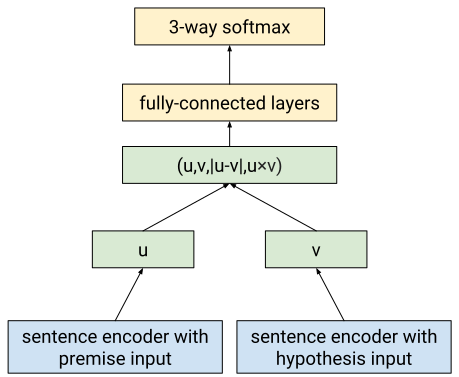
\includegraphics[width=0.5\textwidth,scale=0.5]{images/nli}
	\caption{Generic training scheme of \emph{InferSent}. Six \emph{sentence encoder} variants were tested.  (Adapted from \cite{Conneau:2017aa})}
		\label{fig:infersent}
\end{figure}


The architecture of the neural network is presented in Figure \ref{fig:infersent}. Two separate encoders are used to encode the text and the hypothesis. The embeddings \emph{u} and \emph{v} are combined into a feature vector which contains the concatenation, the element-wise product and the element-wise difference of \emph{u} and \emph{v}. This vector, containing information from both sentences, is then fed into a fully connected layer and a softmax layer which outputs the probabilities of each label.

The authors tested six architectures for the sentence encoder: LSTM (\cite{hochreiter1997long}), GRU (\cite{cho2014properties}), BiLSTM with mean/max pooling (\cite{collobert2008unified}), self-attentive networks (\cite{liu2016learning}, \cite{lin2017structured}) and hierarchical ConvNet (\cite{zhao2015self}). 

Twelve transfer tasks\footnote{For example: binary classification (sentiment analysis, product reviews, subjectivity/objectivity, opinion polarity), multi-class classification (question type), entailment and semantic relatedness, semantic textual similarity, paraphrase detection and caption-image retrieval.} were used to test the quality of the embeddings. For each task and encoder architecture, the embeddings were used as features. Logistic regression was used as the classification algorithm.

The embeddings generated by the BiLSTM with max pooling and an embedding size of 4096 yielded the best accuracy for SNLI and the transfer tasks. Also, the embeddings were better than other state-of-the-art sentence embeddings like SkipThought.

A pretrained model for InferSent is available on GitHub\footnote{\url{https://github.com/facebookresearch/InferSent} (checked: 13.05.2018)}. This model was used in Section \ref{sec:features}.

\subsection{HypeNet and LexNet}
\label{sec:lexnet}
HypeNet, presented in \cite{DBLP:conf/acl/ShwartzGD16}, is a method to detect hypernym relations between words. It combines distributional and dependency path based methods to create a vector representation for sentences, which are used as features for the hypernymy detection. LexNet, presented in \cite{DBLP:journals/corr/ShwartzD16}, is a generalisation of HypeNet, which is able to detect multiple semantic relationships between two words.

The dependency paths add information about joint occurrences of the two words, while the distributional methods add information about the words in separate contexts. Word embeddings are used as distributional features.

For each term pair, all dependency paths were extracted. Each edge was represented as \texttt{lemma/POS/dependency label/direction}. An example is given in Figure \ref{fig:hypenet}. 

\begin{figure}[h]
\centering
\caption{Dependency parse of the example sentence \emph{parrot is a bird}, where the relationship between parrot and bird is of interest. This path is represented as \texttt{X/NOUN/nsubj/< be/VERB/ROOT/- Y/NOUN/attr/>} (Adapted from \cite{DBLP:conf/acl/ShwartzGD16}).}
\label{fig:hypenet}
\includegraphics{images/hypenet_example}
\end{figure}


The paths were encoded using an LSTM. The average of all encoded paths was used as the path information for the word pair. The combination of distributional and path information outperformed state-of-the-art techniques.\newline

The task at hand is different from the detection of semantic relations. The relation of two nouns\footnote{The situation might be different if proper nouns are used as well. Fruit is an hypernym for apple, but not for the company Apple.} with respect to hypernyms is unambiguous. Bird is a hypernym for parrot in all cases. Yet the task is not to search for hypernyms or any other semantic relation. It is not possible to assign the correct class by only looking at the objects. For example, there might be sentences saying that \emph{Python} is better than \emph{Ruby}, while others say it is not.

However, it is expected that the dependency path between the objects of interest adds valuable information. In this thesis, the idea on how to extract and encode paths between two words is reused.



